% Author: Izaak Neutelings (October 2017)
\documentclass[border=3pt,tikz]{standalone}
\usepackage{amsmath} % for \text
\usepackage{tikz}
\usetikzlibrary{patterns}
\usetikzlibrary{backgrounds}
\usetikzlibrary{angles,quotes} % for pic
\tikzset{>=latex} % for LaTeX arrow head

\begin{document}



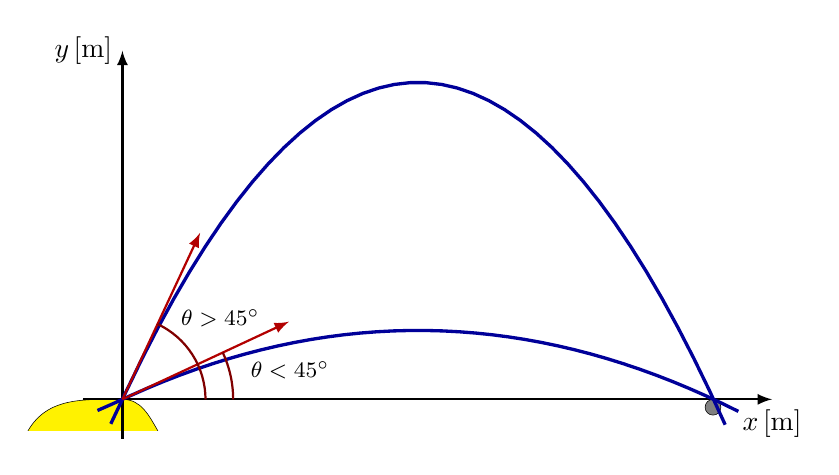
\begin{tikzpicture}[scale=0.5]
  
  \def\N{40}
  \def\vi{14}
  \def\D{15}
  \def\g{10}
  \def\thetaI{65}
  \def\thetaII{25}
  \def\ymax{{\vi^2*sin(\thetaI)^2/(2*\g)*1.1}}
  \def\xmax{\D*1.1}
  \def\xmin{-1}
  \def\ymin{-1}
  \def\tmin{-0.05}
  \def\tmaxI{(2*\vi*sin(\thetaI)/\g)+0.05}
  \def\tmaxII{(2*\vi*sin(\thetaII)/\g)+0.05}
  
  % beach & rock
  \draw[very thin,fill=yellow] %north east lines, crosshatch dots
    (\xmin*2.4,\ymin*0.8) to[out=60,in=180] (0,0) to[out=0,in=120] (-\xmin*0.9,\ymin*0.8);
  \draw[very thin,fill=black!50!white] %north east lines, crosshatch dots
    (\D,-0.2) circle (0.2);
  
  % axes
  \draw[thick,->] (\xmin,0) -- (\xmax,0) node[anchor=north] {$x\,[\text{m}]$};
  \draw[thick,->] (0,\ymin) -- (0,\ymax) node[anchor=east] {$y\,[\text{m}]$};
  
  % parabola
  \draw[very thick,black!40!blue,variable=\t,domain=\tmin:\tmaxI,samples=\N]
    plot ({\vi*cos(\thetaI)*\t},{\vi*sin(\thetaI)*\t-\g*\t^2/2});
  \draw[very thick,black!40!blue,variable=\t,domain=\tmin:\tmaxII,samples=\N]
    plot ({\vi*cos(\thetaII)*\t},{\vi*sin(\thetaII)*\t-\g*\t^2/2});
  
  % vectors
  \coordinate (O)  at (0,0);
  \coordinate (X)  at (1,0);
  \coordinate (V)  at ({\vi*cos(\thetaII)/3},{\vi*sin(\thetaII)/3});
  \coordinate (V') at ({\vi*cos(\thetaI)/3}, {\vi*sin(\thetaI)/3});
  \draw[->,black!30!red,thick] (O) -- (V);
  \draw[->,black!30!red,thick] (O) -- (V');
  
  % angles
  \pic[draw,thick,black!50!red,angle radius=40,angle eccentricity=1.2]
    {angle = X--O--V};
  \pic["\footnotesize$\theta<45^\circ$" right=-4pt,angle radius=40,angle eccentricity=1.2]
    {angle = X--O--V};
  \pic[draw,thick,black!50!red,angle radius=30,angle eccentricity=1.2]
    {angle = X--O--V'};
  \pic["\footnotesize$\theta>45^\circ$" above,angle radius=35,angle eccentricity=1.2]
    {angle = X--O--V'};
  
\end{tikzpicture}



\end{document}